\documentclass[conference,compsoc]{IEEEtran}
\usepackage{amssymb,amsmath,amsthm}
\usepackage{algorithm}
\usepackage{algpseudocode}
\usepackage{graphicx}
\usepackage{caption}
\usepackage{cite}

\newtheorem{theorem}{Theorem}
\newtheorem{definition}{Definition}

\begin{document}

\title{A Branch-and-Cut Algorithm for Constrained Graph Clustering}

\author{\IEEEauthorblockN{Behrouz Babaki}
\IEEEauthorblockA{Dept. Computer Science\\
KU Leuven, Belgium}
\and
\IEEEauthorblockN{Dries Van Daele}
\IEEEauthorblockA{Dept. Computer Science\\
KU Leuven, Belgium}
\and
\IEEEauthorblockN{Tias Guns}
\IEEEauthorblockA{Dept. Business, Technology, \\and Operations\\
VUB, Belgium}}

\maketitle

\begin{abstract}
In this note, we introduce a method for solving a class of graph
clustering problems.
\end{abstract}

\section{Introduction}
\label{introduction}

In this note, we introduce a method for solving a class of graph
clustering problems. The structure of this note is as follows: In
section~\ref{sec:definition} we introduce the problem. In
section~\ref{sec:formulation} we present a mathematical programming
formulation for the problem. This formulation is incomplete in the
sense that the it is not yet clear that how the \emph{connectivity}
constraints will be formulated. In section~\ref{sec:connectivity} we
introduce a formulation for the connectivity constraints. This
formulation involves an exponential number of constraints. We then
present a method for adding only a sufficient subset of these
constraints to the model. We conclude this note in section~\ref{sec:implementation} after 
discussing some of the implementation details.

\section{Probelm definition}
\label{sec:definition}

Consider an undirected graph $G(V, E)$. Our goal is to partition $V$
into $k$ subsets (called \emph{clusters} from now on), such that the
subgraph induced by each subset is connected. Our preference is to avoid
having clusters that contain only a small number of vertices. To enforce
this preference, we define one of our goals as maximizing the size of
the smallest cluster. Moreover, there exists a set of tuples
$C = \{(u, v, w): u, v \in V, w \in \mathbb{R}^+\}$ which indicates that
including $u$ and $v$ in the same cluster will induce a penalty of $w$. We denote all edges $(u, v)$ such that $(u, v, w) \in C$ by $E_C$. Our second goal is to minimize the sum of such penalties.

To include both goals in the objective function, assume that $S$ is the
size of the smallest clsuter and $W$ is the total penalty. We define the
objective function as maximizing $S + \gamma W$ where $\gamma$ is a
parameter specified by user which determines the relative importance of
each of the two goals.

\section{A mathematical programming formulation}
\label{sec:formulation}

We can formulate this problem as an integer linear program. The main
decision variables in this formulation are those that determine the
assignment of vertices to the clusters. In our formulation, the binary
variable $x_{ij}$ indicates whether or not vertex $j$ is included in
cluster $i$. We know that each vertex is assigned to exactly one
cluster. This can be enforced by the following set of constraints:

\begin{equation}
\sum_{i=1}^k x_{ij} = 1 \quad \forall j \in \{1, \ldots, |V|\}
\end{equation}

To include the penalties in the model, we introduce additional
variables. The binary variable $y_{iuv}$ is equal to one if and only if
vertices $u$ and $v$ are both included in the $i$th cluster. To enforce
this property, we add the following constraints to the model:

\begin{equation}
y_{iuv} \geq x_{iu} + x_{iv} -1 \quad \forall i \in \{1, \ldots, k\}, \forall (u, v) \in E_{C}
\end{equation}

If both $x_{iu}$ and $x_{iv}$ are equal to one, this constraint forces
$y_{iuv}$ to be equal to one. Otherwise, $y_{iuv}$ can be either zero or
one. However, as we will see, $y_{iuv}$ is included in the objective
funciton with a negative coefficient. Hence the optimization procedure
will automatically fix $y_{iuv}$ to zero in such cases.

Finally, we introduce an integer variable $s$ which represents the size
of the smallest cluster. The domain of $s$ is
$\{0, \ldots, \lceil \frac{|V|}{k} \rceil \}$. The following constraints
ensure that $s$ represents the size of the smallest cluster:

\begin{equation}
s \leq \sum_{i=1}^{|V|} x_{ij} \quad \forall i \in \{1, \ldots, k\}
\end{equation}

Our formulation so far does not ensure that the vertices in each cluster
are connected. For now assume that constraint
$\mathsf{connected}(x_{i1}, \ldots, x_{i|V|})$ enforces the connectivity of
cluster $i$. We will discuss the exact formulation of this constraint in
the next section. The model that we defined in this section is presented
below:

\begin{align}
& \text{maximize} \quad s + \gamma \sum_{i=1}^{k} \sum_{(w, u, v) \in C} w  y_{iuv}  \\
&\textit{s.t.}                                                                       \nonumber \\
&\sum_{i=1}^k x_{ij} = 1                                                             \forall j \in \{1, \ldots, |V|\} \\
& y_{iuv} \geq x_{iu} + x_{iv} -1                                                    \forall i \in \{1, \ldots, k\}, \forall (u, v) \in E_{C} \\
& s \leq \sum_{i=1}^{|V|} x_{ij}                                                     \forall i \in \{1, \ldots, k\} \\
& \mathsf{connected}(x_{i1}, \ldots, x_{i|V|})                                       \forall i \in \{1, \ldots, k\} \\
& x_{ij} \in \{0, 1\}                                                                \forall i \in \{1, \ldots, k\}, \forall j \in \{1, \ldots, |V|\} \\
& y_{iuv} \in \{0, 1\}                                                               \forall i \in \{1, \ldots, k\}, \forall (u, v) \in E_{C} \\
& s \in \{0, \ldots, \lceil \frac{|V|}{k} \rceil \}                                  
\end{align}

\section{Enforcing connectivity}
\label{sec:connectivity}

In the previous section we did not give a concrete formulation for the constraint $\mathsf{connected}(x_{i1}, \ldots, x_{i|V|})$. In this section we present a method for enforcing this constraint. The contents of this
section are a slight modification of the methods presented in~\cite{CarvajalCGVW13}. The presented formulation of connectivity constraints is mainly based on the notion of \emph{node-cut sets}, which we define next. 

\begin{definition}[Node-cut set]
Given nodes $u, v \in V$ that are not adjacent ($(u, v) \notin E$), a set of nodes $S \subseteq V \setminus \{u, v\}$ is a \emph{node-cut set} separating $u$ and $v$ (or simply a \emph{$uv$-node cut}) if all paths between $u$ and $v$ intersect $S$.
\end{definition}

A $uv$-node cut is \emph{minimal} if it is not a $uv$-node cut after removing any of its vertices. Figures \ref{fig:nodecut} and \ref{fig:minimal} depict the idea of a node-cut. The following theorem shows that connectivity of a graph can be characterized by its node-cut sets. 

\begin{figure}
\centering
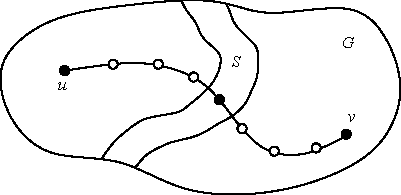
\includegraphics[scale=0.7]{node_cut}
\caption{$S$ is a $uv$-node cut set. Each path between $u$ and $v$ passes through $S$}
\label{fig:nodecut}
\end{figure}

\begin{figure}
\centering
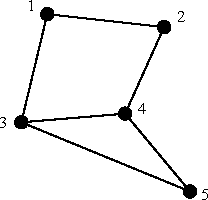
\includegraphics[scale=0.7]{minimal}
\caption{The set \{3, 4\} belongs to $\Gamma(2, 5)$, but the set \{1, 3, 4\} does not.}
\label{fig:minimal}
\end{figure}

\begin{theorem}
Given $U \subseteq V$ and a pair of non-adjacent nodes $u, v \in U$, there exists a path between $u$ and $v$ in the subgraph induced by $U$ if and only if all $uv$-node cuts $S$ are such that $S \cap U \neq \emptyset$.
\end{theorem}

Let us denote by $\Gamma(u, v)$ the set of all minimal $uv$-node cut sets. Then the constraint $\mathsf{connected}(x_{i1}, \ldots, x_{i|V|})$ can be formulated as follows:

\begin{align}
\sum_{w \in S} x_{iw} \geq x_{iu} &+ x_{iv} - 1 \nonumber \\ 
&\forall S \in \Gamma(u, v), \forall (u, v) \in V, (u, v) \notin E
\label{eq:connectivity}
\end{align}

This formulation adds an exponential number of inequalities to the
problem, which makes it impractical for all graphs but those with only a
few vertices. To resolve this problem, we use the \emph{cutting-plane}
method. A rough description of this method follows: We start by
including a (possibly empty) subset of these constraints and solve the
problem to optimality. The we check to see if the solution satisfies the
connectivity constraints. If it does, then this solution is also the
optimal solution for the original problem. Otherwise, we add (some of)
the violated constraints to the problem and repeat this procedure, until
all connectivity constraints are satisfied.

Note that we need a means to detect which constraints are violated by
the current solution. Since we do not want to enumerate an exponential
number of constraints, this question gives rise to another search
problem (called the \emph{separation} problem). The separation problem
is usually formulated as that of finding the \emph{most violated}
constraint.

Luckily, for the connectivity constraints, the separation problem can be
solved efficiently. Given a solution of the problem, the
separation problem for cluster $i$ can be stated as an optimization subproblem: Let us denote the value of $x_{ij}$ variables in this solution by $x^*_{ij}$. Find vertices $u$ and $v$ such that $(u, v) \notin E$ and a set $S^* \in \Gamma(u, v)$ such that the sum $\sum_{w \in S^*} x_{iw}^*$ is
minimum among all sets $S \in \Gamma(u, v)$. If $\sum_{w \in S^*} x_{iw}^* < x^*_{iu} + x^*_{iv} - 1$ then the equality~\ref{eq:connectivity}
induced by $u, v, S^*$ is violated. We solve this separation problem
once for each cluster and add the violated constraints to the problem.
If no such violated constraint is found, then the solution is optimal.

The question is now how to find $S^*$, the minimum node cut separating
$u$ and $v$. We use the following theorem to solve this problem:

\begin{theorem}
Given a graph with node capacities, the maximum flow between
two non-adjacent nodes $u$ and $v$ equals the capacity of the minimum
capacity node cut separating $u$ and $v$.
\end{theorem}

To solve the separation problem, we solve a max-flow problem for each
pair of non-adjacent nodes using values $x^*_{ij}$ as node capacities. We repeat this $k$ times, once for every cluster. This procedure is summarized in algorithm~\ref{alg:cut}.

\begin{algorithm}
\centering
\caption{The cut-generation procedure}
\label{alg:cut}
\begin{algorithmic}
\State $\mathcal{C} \gets \emptyset$
\For{$i \in \{1, \ldots, k\}$}
	\For{$u, v$ such that $(u, v) \notin E$}
		\State $S^* \gets \text{min-cut}(u, v, x^{*i})$ \Comment Find the minimum $uv$-node cut
		\If{$\sum_{w \in S^*} x_{iw}^* < x_{iu}^* + x_{iv}^* - 1$}
			\State $\mathcal{C} \gets \mathcal{C} \cup \{\sum_{w \in S^*} x_{iw} \geq x_{iu} + x_{iv} - 1\}$ \Comment violated constraint
		\EndIf
	\EndFor
\EndFor
\State Add constraints $\mathcal{C}$ to the model
\end{algorithmic}
\end{algorithm}

Now observe that we do not need to wait for the problem to be solved to
optimality to add the violated constraints. Instead, we can do so each
time a feasible solution is found during the branch-and-bound procedure.
We can also take a step further and solve the separation problem using
the solution for the linear relaxation of the problem. We use both these
practices in our implementation.

\section{Implementation details}
\label{sec:implementation}

We implemented our branch-and-cut algorithm using the python interface
of \emph{Gurobi-6.5}\footnote{www.gurobi.com}. To solve the separation problem, we used the
implementation of min-cut/max-flow algorithm from the \emph{NetworkX-1.11}\footnote{networkx.github.io} library. To use this implementation for our problem, we replaced
each undirected edge by two opposite directed edges. The capacity of
these edges is infinite. Then we replaced each vertex $v$ by two
vertices $v_{\text{in}}, v_{\text{out}}$ connected by two opposite
edges, with capacities equal to the capacity of $v$. We obtain the
minimum node cut separating $u$ and $v$ by computing the minimum cut
between $u_{\text{out}}$ and $v_{\text{in}}$ in this graph.

We followed the recipe of~\cite{CarvajalCGVW13} for adding the cuts: We added cuts to the
linear relaxation only at the root node of the branch-and-cut tree.
Moreover, when adding cuts to the relaxation, we monitored the change in
the value of objective function, and stopped adding the cuts if this
value improved less than 5\% for 10 consecutive rounds. Outside the root
node, we called the separation problem only when a feasible solution was
found.

\bibliographystyle{IEEEtran}
\bibliography{references}

\end{document}
